\documentclass[conference]{IEEEtran}
\IEEEoverridecommandlockouts
% The preceding line is only needed to identify funding in the first footnote. If that is unneeded, please comment it out.
\usepackage{cite}
\usepackage{amsmath,amssymb,amsfonts}
\usepackage{algorithmic}
\usepackage{graphicx}
\usepackage{textcomp}
\usepackage{xcolor}
\usepackage{array}
\usepackage{caption}
\usepackage{placeins}
\usepackage{tikz}
\usetikzlibrary{trees, positioning}
\captionsetup[table]{labelsep=space}
\usepackage{url}
\usepackage{tabularx}
\usepackage{array}

\def\BibTeX{{\rm B\kern-.05em{\sc i\kern-.025em b}\kern-.08em
    T\kern-.1667em\lower.7ex\hbox{E}\kern-.125emX}}
\begin{document}

\title{An Adaptive and Personalized Mental Health Chatbot Through Episodic Memory, Contextual Intelligence and Knowledge Grounding\\
% {\footnotesize \textsuperscript{*}Note: Sub-titles are not captured in Xplore and
% should not be used}
% \thanks{Identify applicable funding agency here. If none, delete this.}
}





\author{%
\normalsize
\renewcommand{\arraystretch}{0.9}%

\begin{tabular*}{\textwidth}{@{\extracolsep{\fill}}p{0.31\textwidth}p{0.31\textwidth}p{0.31\textwidth}@{}}

{\centering
1\textsuperscript{st} Ms. Shwetha S\\
\textit{Assistant Professor and Guide}\\
\textit{Computer Science and Engineering}\\
\textit{JSS Science and Technology University}\\
Mysuru, Karnataka, India\\
shwethas@jssstuniv.in\par} &

{\centering
2\textsuperscript{nd} Pranav G N\\
\textit{Computer Science and Engineering}\\
\textit{JSS Science and Technology University}\\
Mysuru, Karnataka, India\\
pranavgn2005@gmail.com\par} &

{\centering
3\textsuperscript{rd} Lathesh Rai M\\
\textit{Computer Science and Engineering}\\
\textit{JSS Science and Technology University}\\
Mysuru, Karnataka, India\\
latheshraikumbra@gmail.com\par}

\\
\noalign{\vskip 2ex}

\multicolumn{3}{c}{%
\begin{tabular}{@{}p{0.31\textwidth}@{\hspace{0.6cm}}p{0.31\textwidth}@{}}

{\centering
4\textsuperscript{th} Aditya Prakash Konnur\\
\textit{Computer Science and Engineering}\\
\textit{JSS Science and Technology University}\\
Mysuru, Karnataka, India\\
adityakonnur@gmail.com\par} &

{\centering
5\textsuperscript{th} Vasudev Mishra\\
\textit{Computer Science and Engineering}\\
\textit{JSS Science and Technology University}\\
Mysuru, Karnataka, India\\
vdmishra004@gmail.com\par}

\end{tabular}%
}

\end{tabular*}%
}




\maketitle

\begin{abstract}
Mental health chatbots often struggle to understand users' experiences, emotions, and behavioural patterns across multiple conversations. They may also lack reliable, grounded information when generating responses. To address these limitations, we propose a personalized mental health chatbot that uses Large Language Models (LLMs) across its core components. The system organizes conversations into episodes, tracks users' moods and reflections, and identifies recurring patterns across past experiences. These are consolidated into long-term memory and used in future interactions, along with the user's background information, to provide more personalized responses. A Knowledge Retrieval component also retrieves relevant information from curated mental health resources to support grounded responses. The individual components are evaluated through dedicated benchmarks to assess their performance. The system uses the GPT-OSS 120B model through the Groq API for LLM-based processing. Its modular design also allows component behaviour to be refined by modifying dedicated prompts, providing flexibility to adapt and improve the system without major changes to its implementation.
\end{abstract}


\begin{IEEEkeywords}
Mental Health Support, Conversational Artificial Intelligence, Personalized Assistance, Episodic Memory, Long-Term Memory, Memory Consolidation, Pattern Detection, Retrieval-Augmented Generation (RAG), Large Language Models (LLMs), FastAPI, ChromaDB
\end{IEEEkeywords}


\section{Introduction}

Mental health concerns such as anxiety, depression, and stress can affect an individual's emotions, behaviour, and daily life. Recent advances in conversational AI have created opportunities for chatbots that allow people to express their thoughts and discuss personal concerns. However, understanding a person requires more than interpreting individual messages. Their emotions, experiences, and concerns develop over time, making continuity across conversations important for meaningful support.

Systems such as Woebot, Wysa, and Replika have explored different approaches to conversational support, while research in affective computing and transformer-based models has advanced emotion recognition and contextual understanding. However, maintaining an understanding of users across multiple conversations remains challenging. Recurring concerns, emotional changes, and behavioural patterns may not be apparent from individual interactions alone [1].

To address this, our work explores a conversational system that uses information from previous interactions to provide more context-aware and personalized responses. By maintaining a record of user experiences and identifying recurring patterns, the system aims to provide continuity across conversations. The proposed approach is also evaluated through component-level testing to examine the performance of its individual modules.

\begin{table*}[!t]
\centering
\renewcommand{\arraystretch}{1.5}
\begin{tabular}{|m{2.8cm}|m{3.1cm}|m{4.2cm}|m{5cm}|}
\hline
\centering\arraybackslash\textbf{Study} &
\centering\arraybackslash\textbf{Approach} &
\centering\arraybackslash\textbf{Key Features} &
\centering\arraybackslash\textbf{Comparison with Proposed System} \\
\hline

Jaybhaye et al. \cite{b2} &
NLP and machine learning &
Mental health education, psychoeducation, resource delivery and conversational support. &
Focuses on mental health education, whereas the proposed system emphasizes episodic context and long-term personalization. \\
\hline

Subash et al. \cite{b3} &
NLP and sentiment analysis &
Tracks mood fluctuations, identifies distress patterns and provides personalized support. &
Includes mood tracking and pattern detection, while the proposed system additionally organizes experiences into episodes and consolidates insights into long-term memory. \\
\hline

Verma et al. \cite{b4} &
BERT, emotion detection and reinforcement learning &
Uses emotional analysis, CBT techniques and previous interactions to adapt responses. &
Uses interaction history for personalization, whereas the proposed system employs dedicated episodic memory, pattern identification and memory consolidation. \\
\hline

Sophia et al. \cite{b5} &
BERT, BART and RAG &
Uses a vector database for knowledge retrieval and evaluates generated responses using BLEU, ROUGE and other metrics. &
Focuses on knowledge retrieval and response generation, while the proposed system also maintains personalized context through a separate memory retrieval mechanism. \\
\hline

Nair et al. \cite{b6} &
Agentic AI, RAG and knowledge graphs &
Combines emotion detection, condition-specific agents and memory-based personalization. &
Closely related in memory-based personalization and knowledge retrieval. The proposed system emphasizes episode management, reflection tracking, recurring pattern identification and memory consolidation. \\
\hline

Mavila et al. \cite{b8} &
Rasa, NLP, machine learning and LLM fallback &
Uses therapist-response datasets, intent classification and GPT-3 fallback to generate empathetic responses. Stores conversation history for registered users. &
Uses conversation history and an LLM fallback, whereas the proposed system employs structured episodic memory, cross-episode pattern identification and long-term memory consolidation. \\
\hline

\textbf{Proposed System} &
LLM-based processing with episodic memory and RAG &
Mood tracking, reflection tracking, pattern identification, memory consolidation and knowledge retrieval. &
Integrates accumulated personal experiences with external knowledge to support continuous and personalized conversations. \\
\hline

\end{tabular}
\caption{Comparison of Existing Mental Health Chatbot Systems}
\label{tab:literature}
\end{table*}

\begin{table*}[!t]
\centering
\scriptsize
\renewcommand{\arraystretch}{1.4}
\setlength{\tabcolsep}{5pt}

\begin{tabular}{|
>{\centering\arraybackslash}p{0.15\textwidth}|
>{\centering\arraybackslash}p{0.15\textwidth}|
>{\centering\arraybackslash}p{0.15\textwidth}|
>{\centering\arraybackslash}p{0.15\textwidth}|
>{\centering\arraybackslash}p{0.15\textwidth}|
>{\centering\arraybackslash}p{0.15\textwidth}|}
\hline

\textbf{Feature} &
\textbf{Wysa} &
\textbf{Therabot} &
\textbf{Woebot} &
\textbf{AIMind} &
\textbf{Proposed System} \\
\hline

Deployment &
Cloud &
Cloud &
Cloud &
Cloud &
Cloud-based \\
\hline

Data Privacy &
Policy Protected &
Policy Protected &
Policy Protected &
Federated Learning &
Secure Data Storage \\
\hline

External Emotions &
No &
Limited &
No &
Yes &
Yes \\
\hline

Emotion Model &
Rule + ML Classifier &
Generative Context &
Rule-Based &
Multi-label External Emotions &
LLM-based Mood Analysis \\
\hline

Crisis Escalation &
Limited &
Human-AI Hybrid &
Limited &
Mandatory &
Safety Detection \\
\hline

Long-Term Memory &
Single Session &
Multi-session Window &
Single Session &
Compressed Context Summaries &
Episodic and Long-Term Memory \\
\hline

Cultural Adaptability &
Low &
Medium &
Low &
High &
Context-dependent \\
\hline

Explainability &
No &
No &
No &
Yes &
Evidence-based Context Retrieval \\
\hline

\end{tabular}
\caption{Feature Comparison of Existing Mental Health Chatbots and the Proposed System \cite{b7}}
\label{tab:chatbot_comparison}
\end{table*}

\section{Literature Review}
Recent studies have explored conversational AI for mental health support using techniques such as NLP, sentiment analysis, machine learning, and LLMs. Table~\ref{tab:literature} compares these approaches and their relevance to the proposed system..

Existing mental health chatbots also differ in their features, particularly in areas such as emotion detection, memory, privacy, and crisis management. Table~\ref{tab:chatbot_comparison} compares selected platforms based on these capabilities, highlighting the differences between their approaches.

Jewell et al. \cite{b9} proposed a framework for organizing memory in AI-powered mental health systems to support continuity across interactions. The framework identifies four types of memory: episodic memory for recording specific experiences, pattern memory for identifying recurring cognitive, emotional and behavioral patterns, semantic memory for retaining stable user information, and state-responsive memory for representing the user's current condition. The authors emphasize that memory should support longitudinal understanding rather than serve only as a personalization mechanism. This work is closely related to the proposed system's use of episodic memory, pattern identification and long-term memory consolidation.

`
Hao et al. \cite{b10} discussed the limitations of LLMs in retaining information across sessions and using past experiences in future interactions. They proposed the Episodic-Augmented Large Language Model (EALLM), which uses episodic memory to store and retrieve past experiences. Their work also describes consolidating these experiences into higher-level representations to identify recurring patterns. These ideas provide a theoretical basis for the proposed system's episodic memory, pattern identification, and long-term memory consolidation.

Leung et al. \cite{b11} reviewed eight randomized controlled trials involving 921 participants to assess chatbot-based mental health interventions in Asian populations. Their findings showed a significant reduction in depressive symptoms, but no significant overall effects on anxiety, stress, and several other outcomes. The study highlights the potential of chatbots as accessible mental health support tools.

These studies highlight the potential of mental health chatbots while emphasizing the need for better continuity and personalization across conversations.

\section{Proposed Methodology}

\subsection{Proposed System Workflow}
The proposed system follows a two-stage workflow: real-time response generation and continuous learning through memory management. These stages work together to provide context-aware and personalized mental health support across conversations.

\begin{figure}
    \centering
    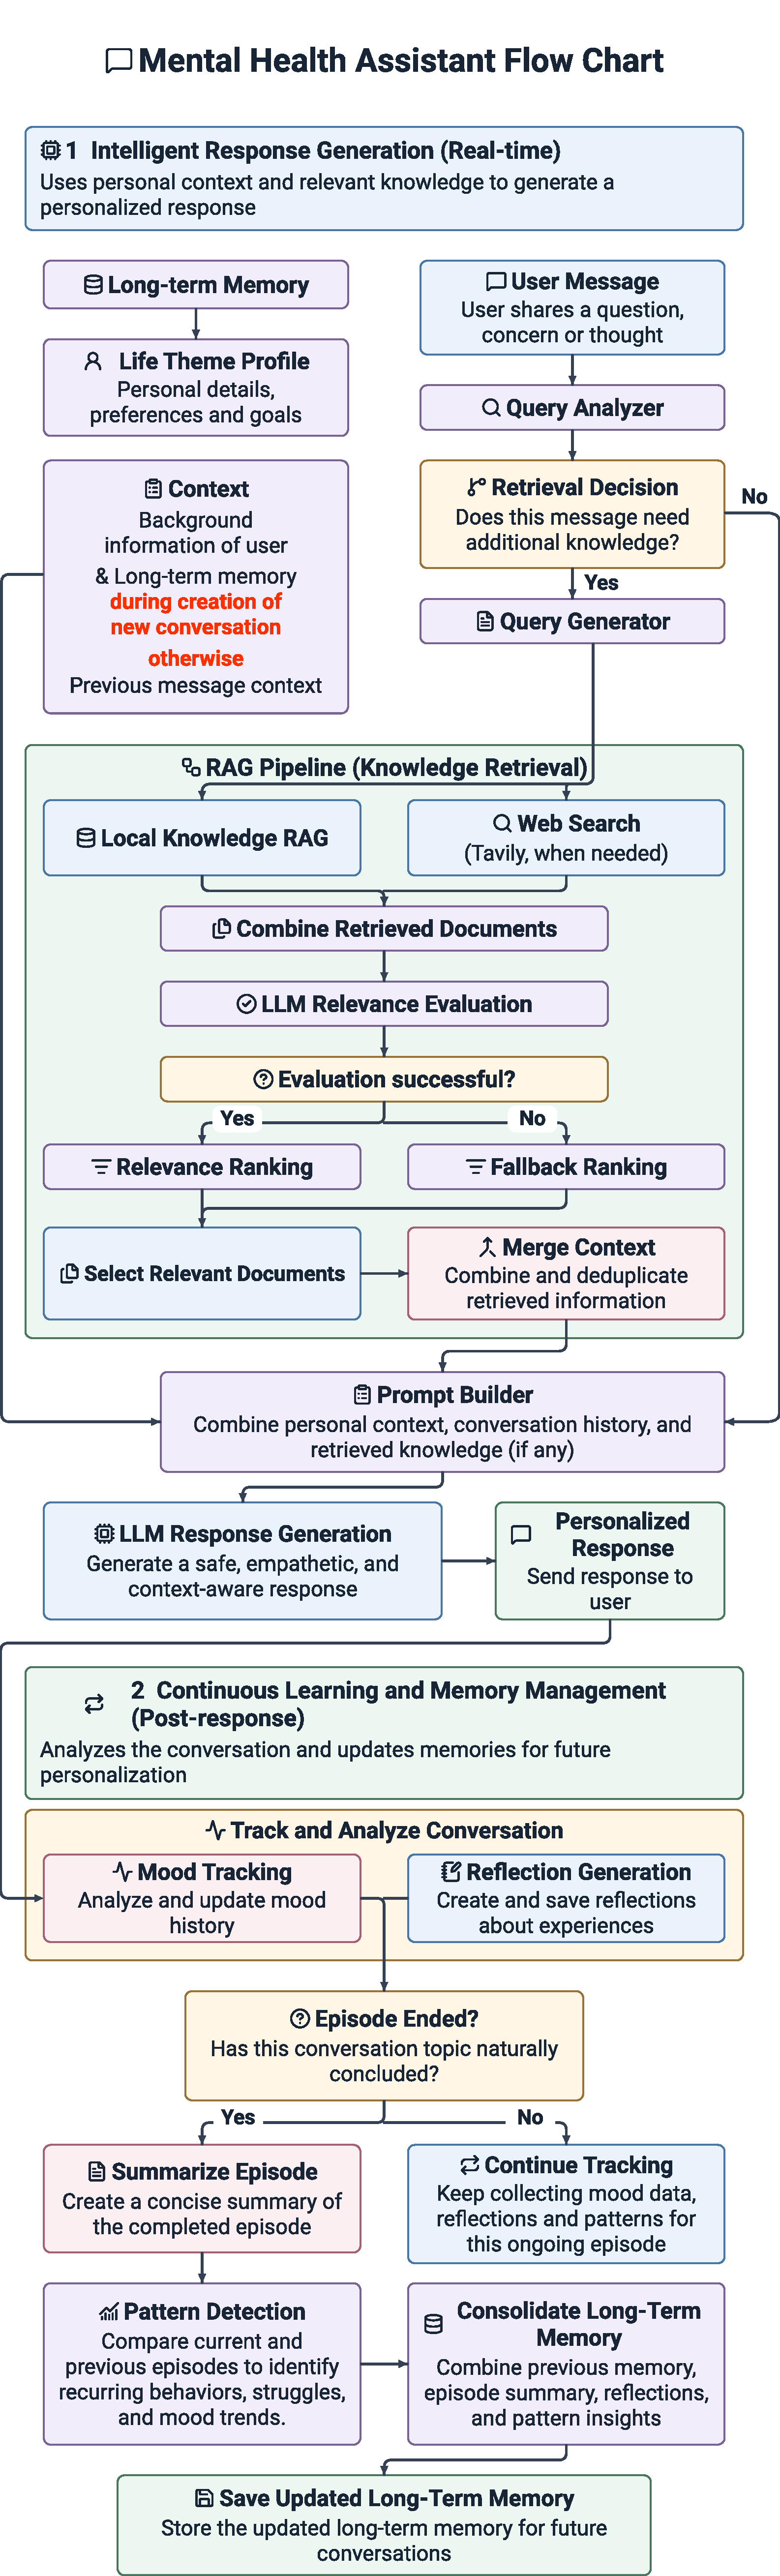
\includegraphics[width=0.76\linewidth]{Mental Health Assistant Flow Chart.pdf}
    \caption{Workflow of the proposed system, showing response generation and memory management.}
    \label{fig:placeholder}
\end{figure}

At the beginning of a new conversation, the system retrieves the user's background information and existing long-term memory to establish the initial context. If the conversation is identified as mental health-related and no active episode exists, a new episode is initiated to organize the interaction.

 \subsubsection{Intelligent Response Generation}

When a user sends a message, the system first analyzes the query to determine whether additional knowledge is required. If needed, relevant information is retrieved through the Knowledge RAG pipeline. This pipeline uses a local knowledge base and web search when necessary. The retrieved documents are then evaluated for relevance, ranked, and selected for use.

During subsequent turns, the previous messages in the conversation are included as context to maintain continuity, similar to how conversational context is handled in ChatGPT \cite{chatgpt}. The prompt builder combines this information with the retrieved knowledge, when available, and passes it to the LLM. The LLM then generates a response based on the current message and the available context.

\subsubsection{Continuous Learning and Memory Management}

After generating a response, the system analyzes the conversation to update the user's mood history and identify reflections about their experiences. It also monitors the conversation to determine whether the current episode has reached its endpoint.

If the episode is still ongoing, the system continues tracking the interaction. Once an episode ends, a summary is generated. The system then compares it with previous episodes to identify recurring behaviors, struggles, and mood patterns.

The identified patterns and relevant reflections are then combined with existing long-term memory during the memory consolidation process. The updated memory is stored and made available for future conversations. This allows information from previous interactions to contribute to the context of subsequent conversations.

\subsubsection{Interaction Between System Components}

The response generation and memory management processes work together in a continuous cycle. Previous interactions provide context for current responses, while new conversations contribute to the system's evolving memory. This enables the chatbot to maintain continuity and provide more personalized support over time.

\subsection{Frontend Application Interface}

The system provides a web-based interface built with React, featuring login and registration pages, a chat interface, and a sidebar for managing conversations (Fig.~2). A dedicated \textbf{Your Account} panel allows users to view their profile, personal details, episodes, mood history, reflections, recurring patterns, and long-term memory (Figs.~3--11). Users can also review and edit supported memory information, giving them access to the data retained from previous interactions.

The frontend uses the following technologies:
\begin{itemize}
    \item \textbf{React and Vite:} Used for interface development and building.
    \item \textbf{React Router and Axios:} Handle page navigation and backend communication.
    \item \textbf{Lucide React:} Provides interface icons.
    \item \textbf{React Markdown and KaTeX:} Display formatted responses and mathematical expressions.
\end{itemize}
The application screenshots are presented below.
\begin{figure}
    \centering
    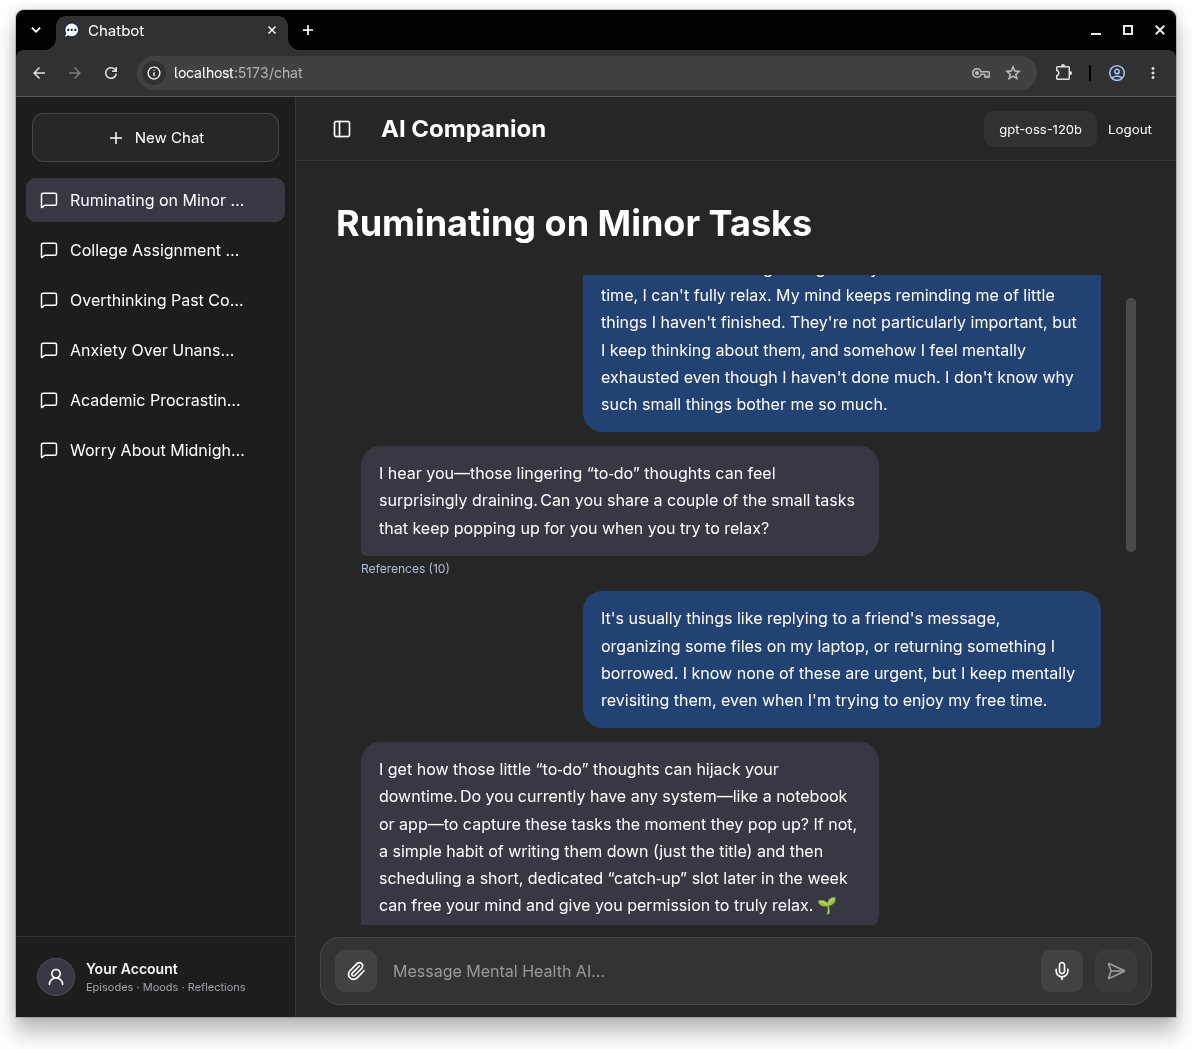
\includegraphics[width=0.8\linewidth]{Chat.png}
    \caption{Chat interface}
    \label{fig:chat}
\end{figure}

\begin{figure}
    \centering
    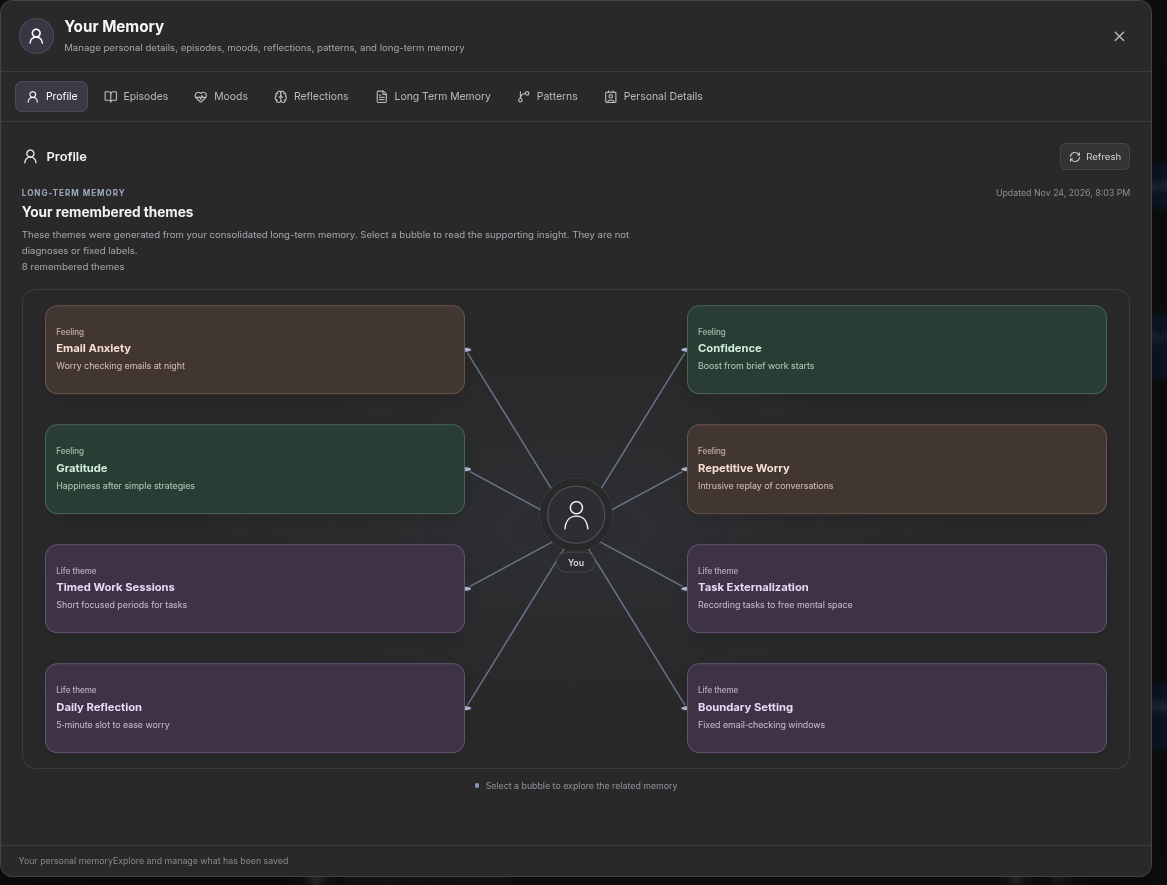
\includegraphics[width=0.9\linewidth]{profile story.png}
    \caption{Profile Themes interface}
    \label{fig:profile-story}
\end{figure}

\begin{figure}
    \centering
    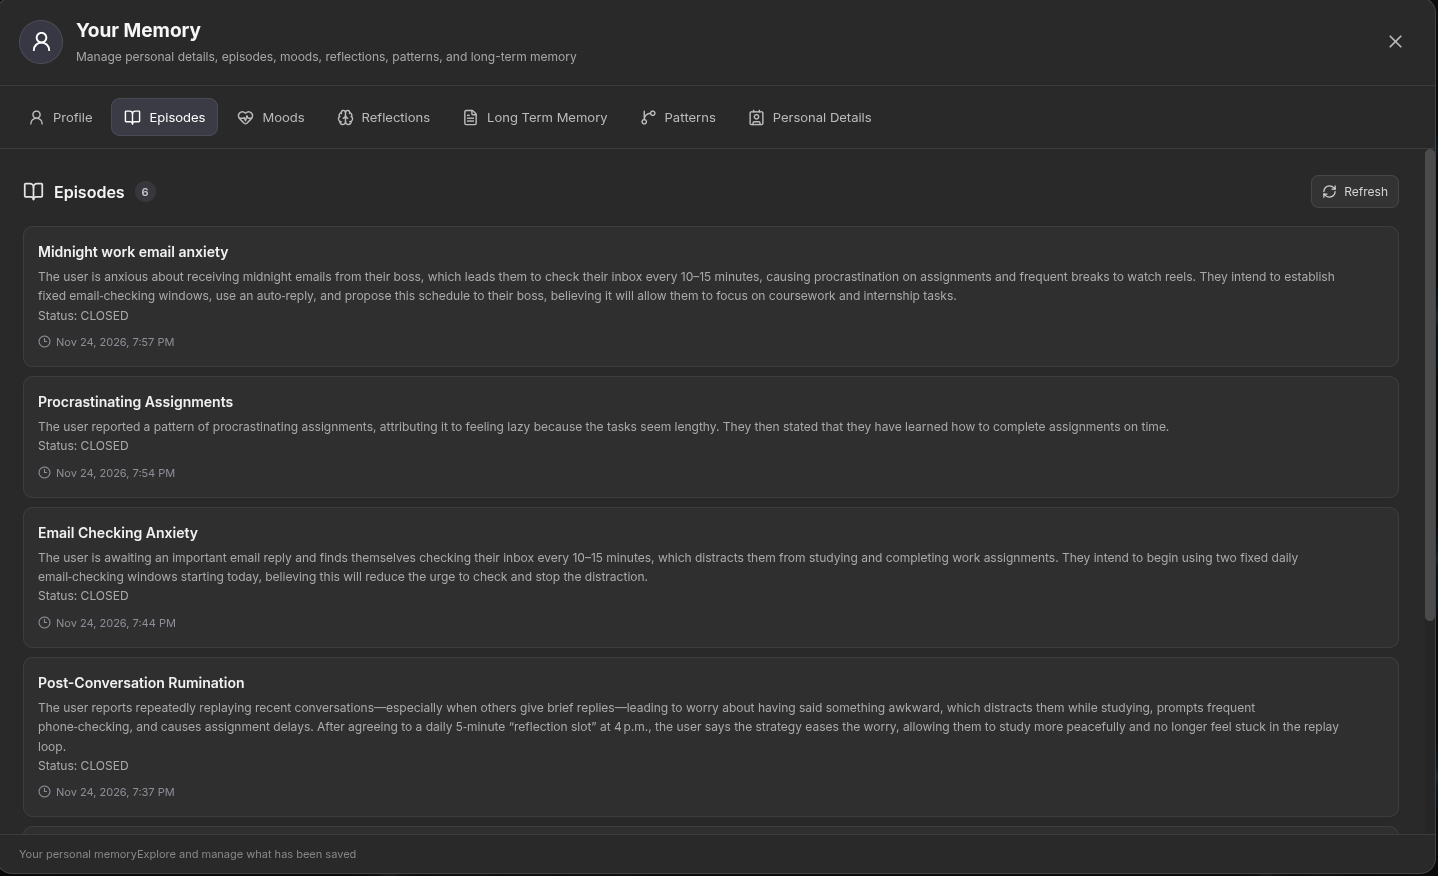
\includegraphics[width=1\linewidth]{Episode_tab.png}
    \caption{Episode manager interface}
    \label{fig:episode_tab}
\end{figure}

\begin{figure}
    \centering
    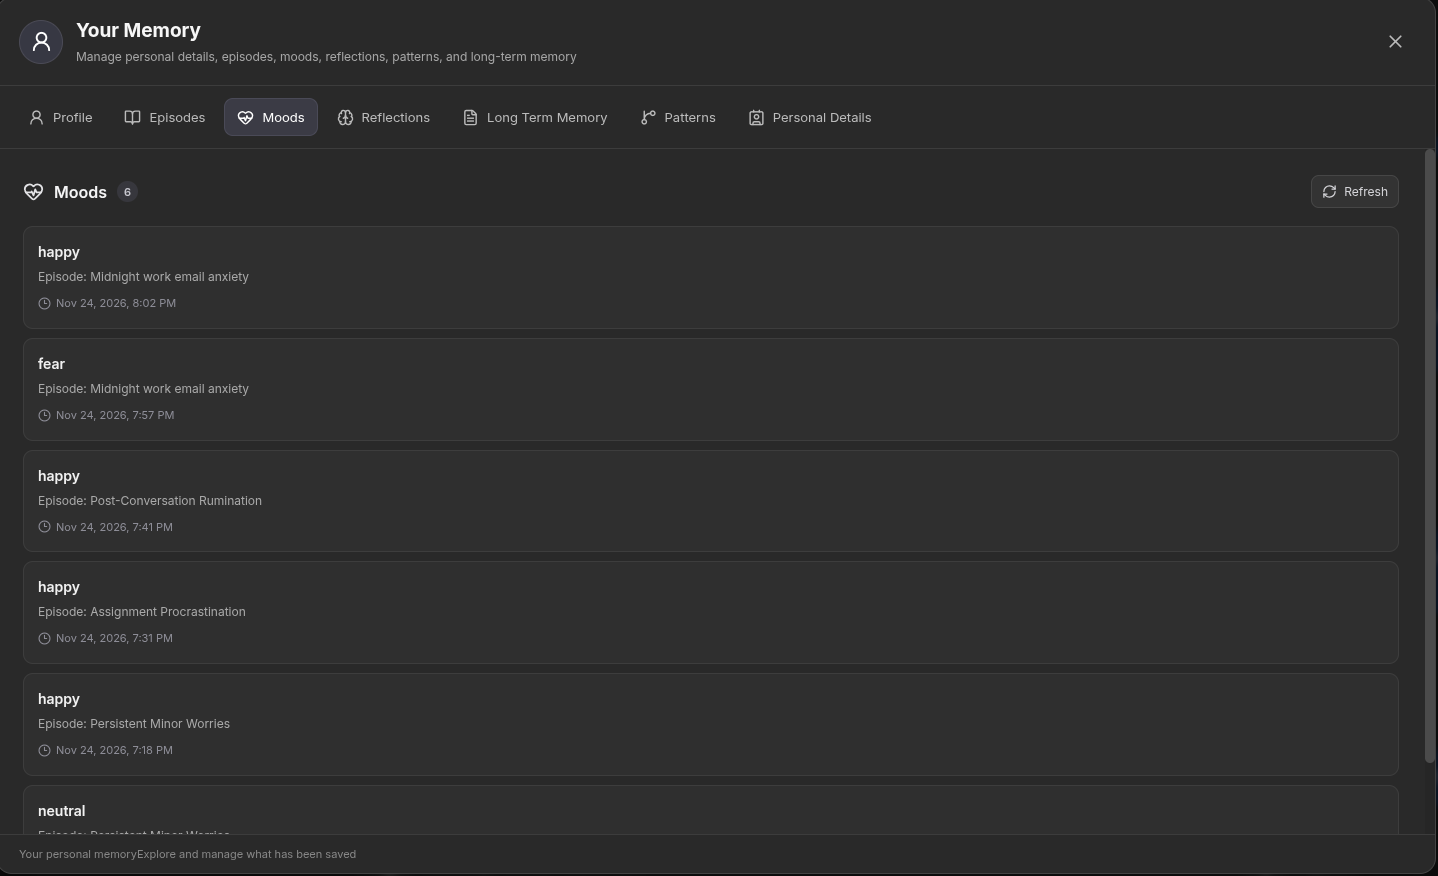
\includegraphics[width=1\linewidth]{mood.png}
    \caption{Mood management interface}
    \label{fig:mood}
\end{figure}

\begin{figure}
    \centering
    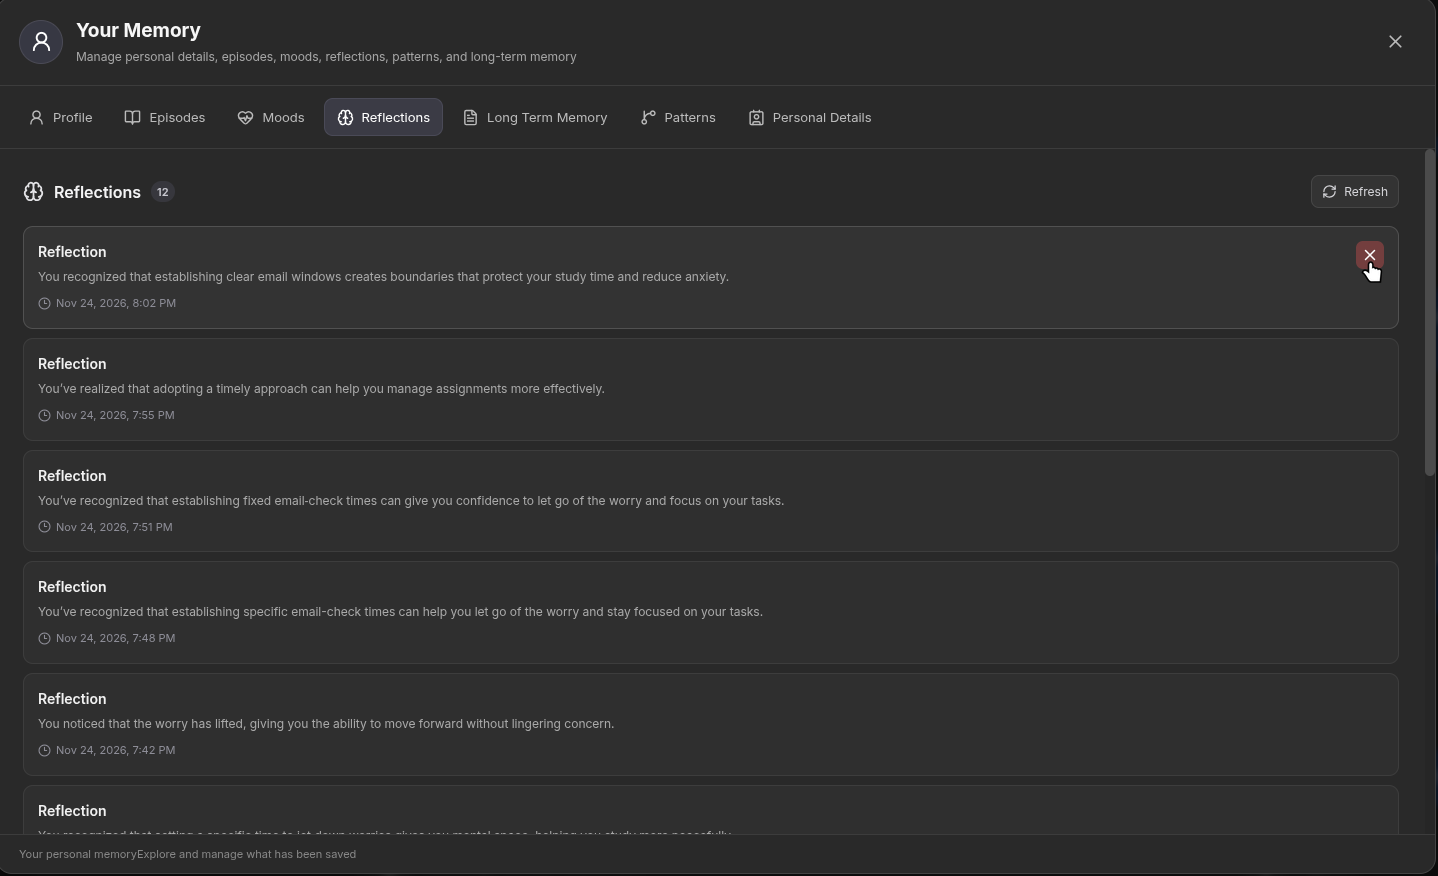
\includegraphics[width=1\linewidth]{Reflection management tab.png}
    \caption{Reflection management interface}
    \label{fig:reflection management tab}
\end{figure}

\begin{figure}
    \centering
    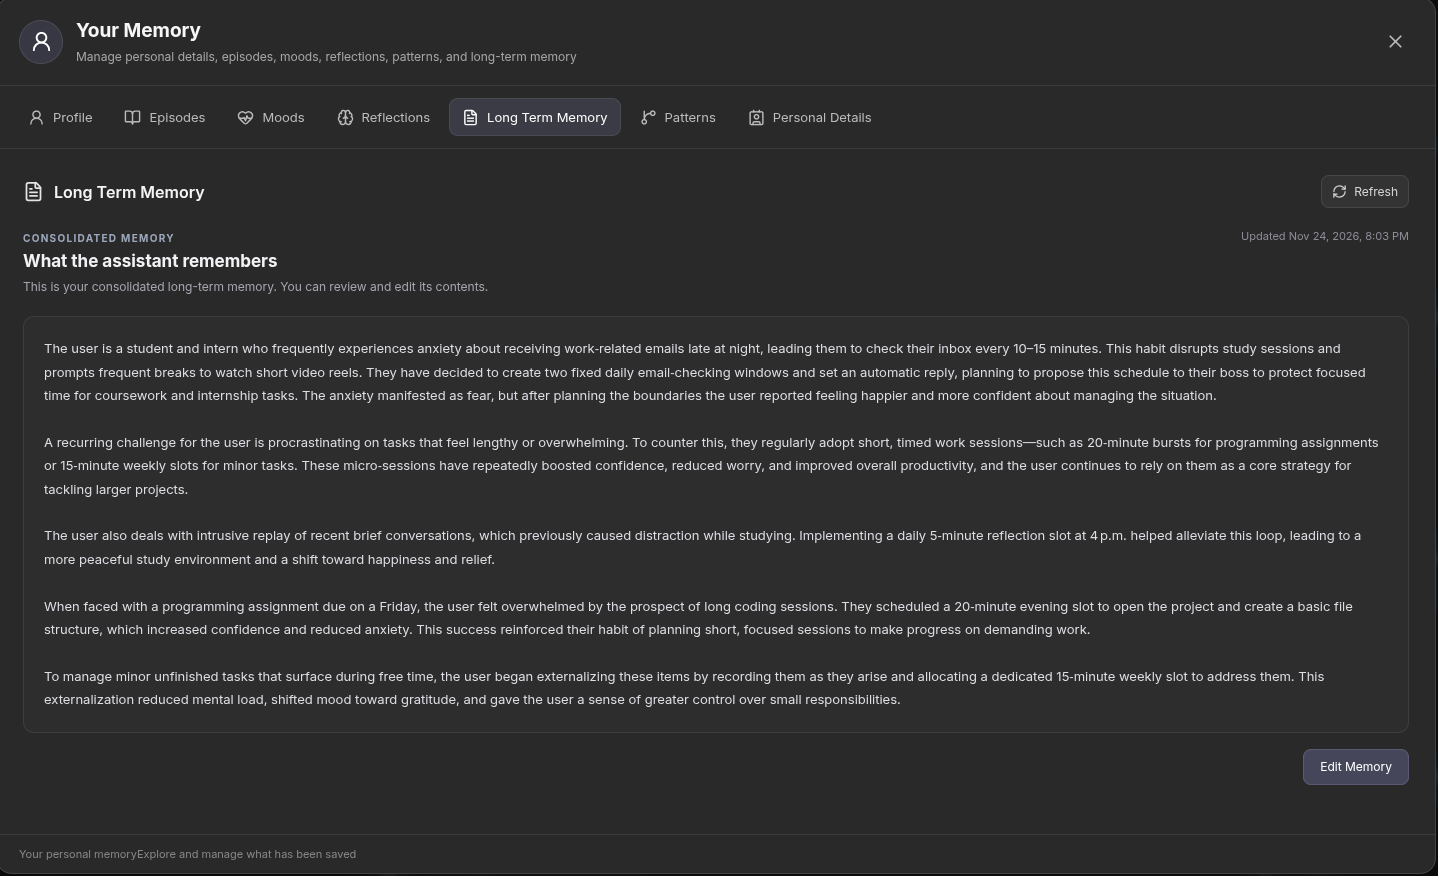
\includegraphics[width=1\linewidth]{Long term memory tab.png}
    \caption{Long term memory management interface}
    \label{fig:long term memeory tab}
\end{figure}

\begin{figure}
    \centering
    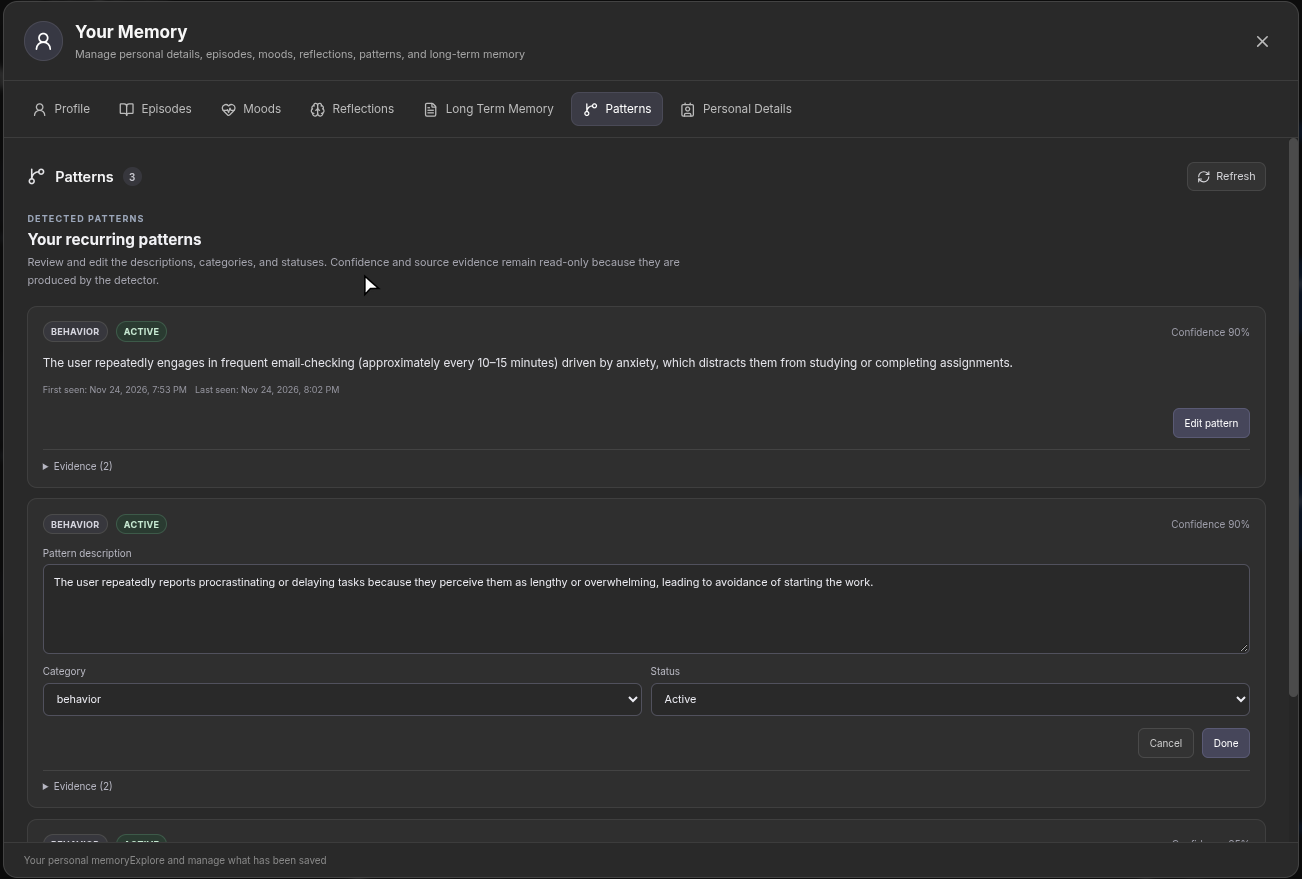
\includegraphics[width=1\linewidth]{Pattern management tab.png}
    \caption{Pattern management interface}
    \label{fig:pattern management}
\end{figure}

\begin{figure}
    \centering
    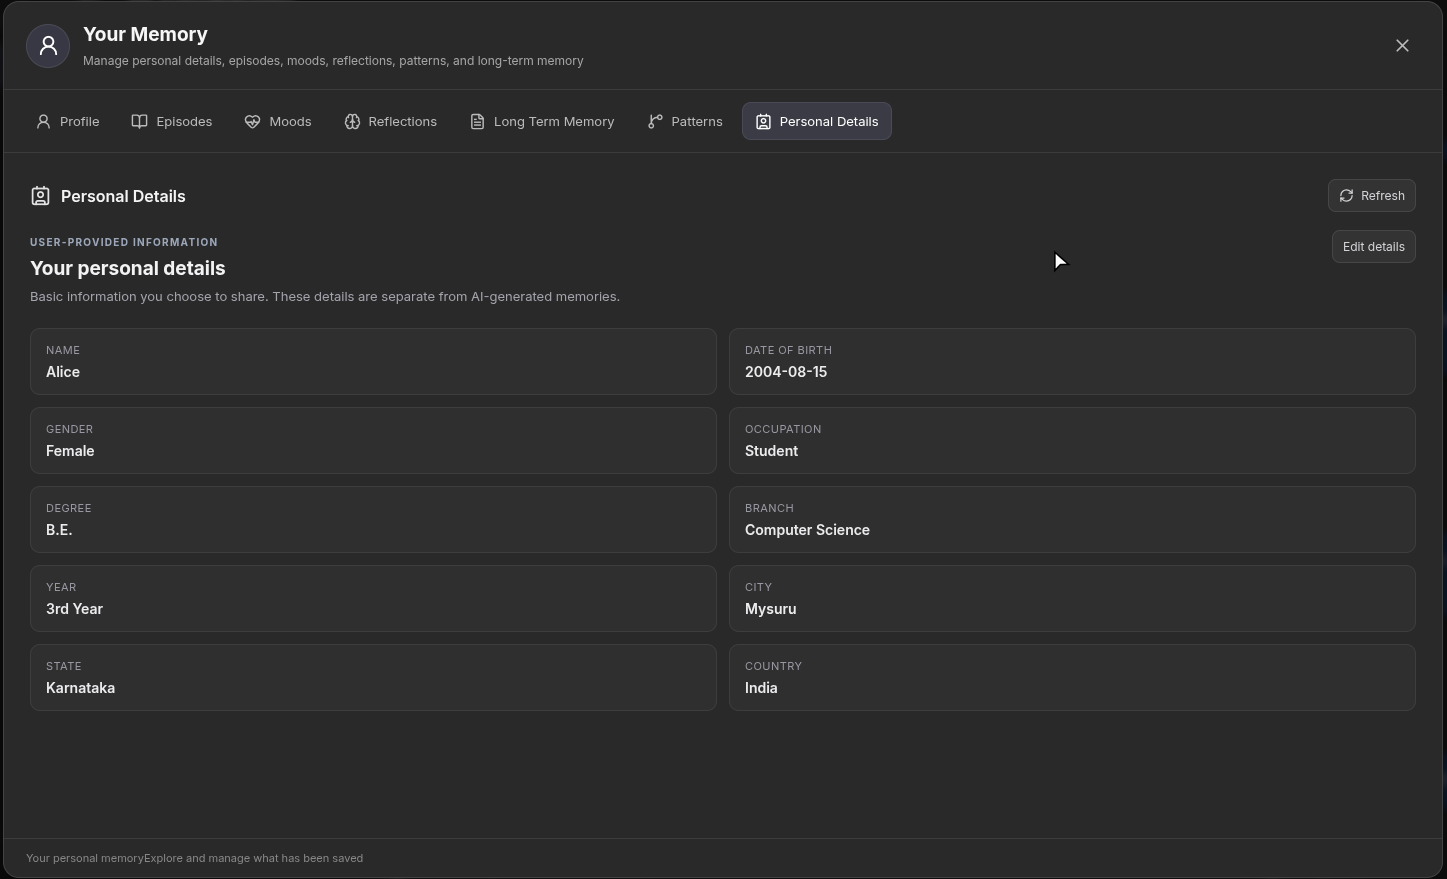
\includegraphics[width=1\linewidth]{personal details tab.png}
    \caption{Personal details management interface}
    \label{fig:personal details}
\end{figure}

\subsection{Backend Technologies}

The backend was developed using the following technologies and libraries:

\begin{itemize}
    \item \textbf{Python and FastAPI:} Python is used for backend development, while FastAPI provides REST APIs for authentication, conversations, memory management, document processing, and response streaming.

    \item \textbf{Pydantic and SQLAlchemy:} Used for API data validation and database operations through an ORM.

    \item \textbf{MySQL and PyMySQL:} Used to store user accounts, conversations, messages, and memory-related data.

    \item \textbf{Groq API:} Provides access to the \textbf{GPT-OSS 120B} \cite{gpt_oss} model for response generation and other LLM-based tasks.\cite{groq} 

    \item \textbf{ChromaDB and Sentence Transformers:} ChromaDB stores document embeddings, while \textbf{BAAI/bge-small-en-v1.5} generates embeddings for semantic retrieval.

    \item \textbf{BM25 and RRF:} Used together with vector search to implement hybrid document retrieval.

    \item \textbf{Tavily Search API:} Retrieves external information when web search is enabled.

    \item \textbf{Docling and HybridChunker:} Used to extract document content and divide it into chunks while retaining structural information such as headings and tables. Hugging Face Transformers provides tokenizer support.

    \item \textbf{PyMuPDF, PyPDF and python-docx:} Used for PDF processing and text extraction from uploaded PDF and DOCX files.

    \item \textbf{python-jose and Passlib:} Used for JWT authentication and password hashing.

    \item \textbf{Uvicorn and Server-Sent Events (SSE):} Uvicorn runs the FastAPI application, while SSE streams chatbot responses to the frontend.
\end{itemize}


\subsection{Backend Architecture and Core Components}

The backend follows a modular architecture, with separate components for response generation, knowledge retrieval, mood tracking, and memory management, coordinated through a central orchestrator. LLM-based operations use dedicated prompts that can be modified to refine individual components. The design also allows different models and providers to be integrated with minimal changes. The backend directory structure is shown in Fig.~12, followed by the implementation details of its core components.

\subsubsection{User Query Processing and Retrieval Routing}
When a user sends a message, the \textbf{Query Analyzer} checks whether additional knowledge is needed. It handles empty messages and predefined immediate-danger phrases separately, while ordinary conversations bypass retrieval. For other queries, it identifies information-seeking requests, requests for current information, and document references.

An LLM then decides whether to use the local knowledge base, web search, or both, with a completion limit of 256 tokens. Web retrieval is disabled by default and controlled through \texttt{RAG\_ENABLE\_WEB}. If the analysis fails, predefined phrases and search cues are used as a fallback.

The \textbf{Query Generator} prepares up to 8 search queries, including the original query. It identifies document references, such as section numbers and table references, and matches them against the indexed knowledge base to create targeted queries. If no matching identifiers are found, an LLM generates one additional query, with a completion limit of 192 tokens. If generation fails, the original query is retained. The resulting queries are passed to the Knowledge RAG pipeline.

\begin{figure}[!t]
\centering
\setlength{\fboxsep}{4pt}
\setlength{\fboxrule}{0.4pt}

\begin{minipage}{\columnwidth}
\raggedright

\textbf{Backend}\par\vspace{2pt}
\fbox{
\begin{minipage}{\dimexpr\columnwidth-2\fboxsep-2\fboxrule\relax}
\scriptsize
\textbf{Core:} main, auth, models, database\\
\textbf{routers/:} auth, chats, messages, memory, profile\\
\textbf{services/:} orchestrator, prompt builder, LLM\\
\textbf{services/ai/:} turn analyzer, episode manager, mood,
reflection, pattern and memory components\\
\textbf{ai/rag/:} query analyzer, query generator, retrievers,
relevance evaluator, context selector\\
\textbf{prompts/:} AI and RAG prompts\\
\textbf{Other:} schemas/, scripts/, benchmark/, knowledge/
\end{minipage}
}

\vspace{4pt}

\textbf{Frontend}\par\vspace{2pt}
\fbox{
\begin{minipage}{\dimexpr\columnwidth-2\fboxsep-2\fboxrule\relax}
\scriptsize
\textbf{src/:} App.jsx, main.jsx\\
\textbf{components/:} ChatWindow, MessageBubble, Sidebar, ProfileForm\\
\textbf{pages/:} Chat, Login, Register\\
\textbf{services/:} API, authentication, chat, messages\\
\textbf{context/:} AppContext\\
\textbf{hooks/:} useChat\\
\textbf{styles/:} CSS files
\end{minipage}
}

\end{minipage}

\caption{Simplified project directory structure.}
\label{fig:directory_structure}
\end{figure}

\subsubsection{Knowledge Retrieval, Relevance Evaluation and Context Selection}

The \textbf{Knowledge RAG Pipeline} retrieves relevant information using the generated search queries. Local retrieval combines semantic search through \textbf{ChromaDB} and keyword-based search using \textbf{BM25}. Their results are merged using \textbf{Reciprocal Rank Fusion (RRF)}, with a default limit of 12 results per query and an RRF constant of 60. Documents matching explicitly requested identifiers, such as section numbers and recommendation references, receive an additional ranking boost. When enabled, the \textbf{Tavily Search API} retrieves information from external sources. Web retrieval is disabled by default, and local and web retrieval run concurrently when both are selected.

The retrieved documents are evaluated by the \textbf{Relevance Evaluator} using a weighted score based on retrieval relevance (45\%), keyword overlap (30\%), and identifier coverage (20\%). An additional 5\% is applied when evidence-related information is relevant to the query. Optional LLM-based reranking can further refine the results but is disabled by default. When enabled, the final score combines the deterministic and LLM scores with weights of 75\% and 25\%, respectively.

Finally, the \textbf{Context Selector} prioritizes documents containing requested identifiers, followed by those with higher relevance scores. Duplicate content is removed, and the selection is limited to 10 chunks and 16,000 characters by default. Complete chunks are preserved without truncation to retain important information, particularly in structured tables. The selected content is formatted with available source details, such as document titles, page numbers, and URLs, and passed to the LLM as additional context.

\subsubsection{Preparation, Prompt Building and Response Generation}
Once the relevant information has been retrieved, the system prepares the context for response generation. This includes the user's profile information, relevant long-term memories, and previous messages from the current conversation. The \textbf{Prompt Builder} combines these details with the retrieved knowledge, when available, and the current user message to construct the prompt for the LLM. The prompt also contains instructions that guide the chatbot to maintain a supportive tone, consider the user's context, and avoid unsupported or inappropriate advice. The prompt is then passed to the \textbf{LLM}, which generates a response based on the information provided. The generated response is returned to the user through the chat interface, taking into account both the ongoing conversation and relevant information from previous interactions.

\subsubsection{Mood Tracking, Reflection and Episode Management}
The \textbf{Turn Analyzer} performs mood classification, reflection generation, and episode lifecycle analysis in a single LLM call for each user turn. It considers the latest message along with up to 8 previous conversation messages, 5 recent mood entries, and 5 previous reflections from the active episode. For mood tracking, it classifies the user's expressed mood into one of 7 categories: happy, sad, angry, fear, disgust, surprise, and neutral. A mood is accepted only when its confidence score is at least 0.75 and supporting evidence is provided. Valid mood entries are linked to the corresponding user message and stored in the database.

The analyzer also generates a reflection when it identifies a meaningful personal insight or realization. Reflections are limited to 2,000 characters, and duplicate consecutive entries are skipped before saving. For episode management, it returns one of four decisions: \textbf{CREATE}, \textbf{CONTINUE}, \textbf{CLOSE}, or \textbf{NONE}. These decisions determine whether a new episode should be created, an existing one should remain active, or the interaction should not be associated with an episode. When an episode is closed, the \textbf{Episode Summarizer} processes its conversation transcript, including both user and assistant messages, to generate a summary of 2--4 sentences with a maximum of 85 words. If the generated summary does not meet these requirements, the system retries generation once. After a valid summary is saved, it is used for long-term memory consolidation. The episode is then marked as closed, even if the optional summarization or memory update process fails.

\subsubsection{Pattern Detection and Long-Term Memory Consolidation}
After an episode is summarized, the \textbf{Pattern Memory Analyzer} compares it with up to 8 previous closed episodes to identify recurring behaviours, triggers, coping strategies, and mood-related patterns. A pattern requires evidence from at least 2 distinct episodes. The analyzer can generate up to 5 new or updated patterns, with a maximum of 10 stored patterns. Each pattern includes supporting evidence and an ACTIVE or RESOLVED status.

The \textbf{Long-Term Memory} component combines the previous memory with the current episode summary, mood observations, reflections, and validated patterns. An LLM generates an updated memory, removing repeated or outdated information while retaining useful details. The updated memory is stored in the database, with a maximum length of 12,000 characters. If consolidation fails, the previous memory is retained.

After consolidation, the \textbf{Profile Generator} analyzes the updated memory along with previously generated themes to identify up to 8 meaningful aspects of the user's experiences. These are categorized as \textit{Feeling} or \textit{Life theme}, with a short title, summary, and supporting details. The generated themes are saved and displayed in the \textbf{Your Memory} interface as connected bubbles around a central user icon. Users can select individual bubbles to view their supporting details, as shown in Fig.~\ref{fig:profile-story}.



\section{Results AND Discussion}
\subsection{Performance evaluation}
The GPT-OSS 120B model used in this work has been evaluated by OpenAI across several established benchmarks covering reasoning, mathematical problem-solving, coding, tool use, and health-related knowledge. The corresponding benchmark results and evaluation details are provided in the official GPT-OSS Model Card \cite{gpt_oss}.
\subsubsection{Hybrid Benchmarking Framework}
The benchmarking framework uses ChatGPT \cite{chatgpt} to generate synthetic datasets containing test inputs and their corresponding expected outputs. These datasets are passed through the system under evaluation to obtain predicted outputs, which are assessed using two complementary approaches: deterministic evaluation through string matching and rule-based checks, and LLM-based evaluation for semantic correctness and contextual relevance. The evaluation results are then aggregated to calculate performance metrics such as Precision, Recall, F1-score, and Accuracy as illustrated in Fig.~\ref{fig:hybrid_benchmark_flowchart}
\begin{figure}
    \centering
    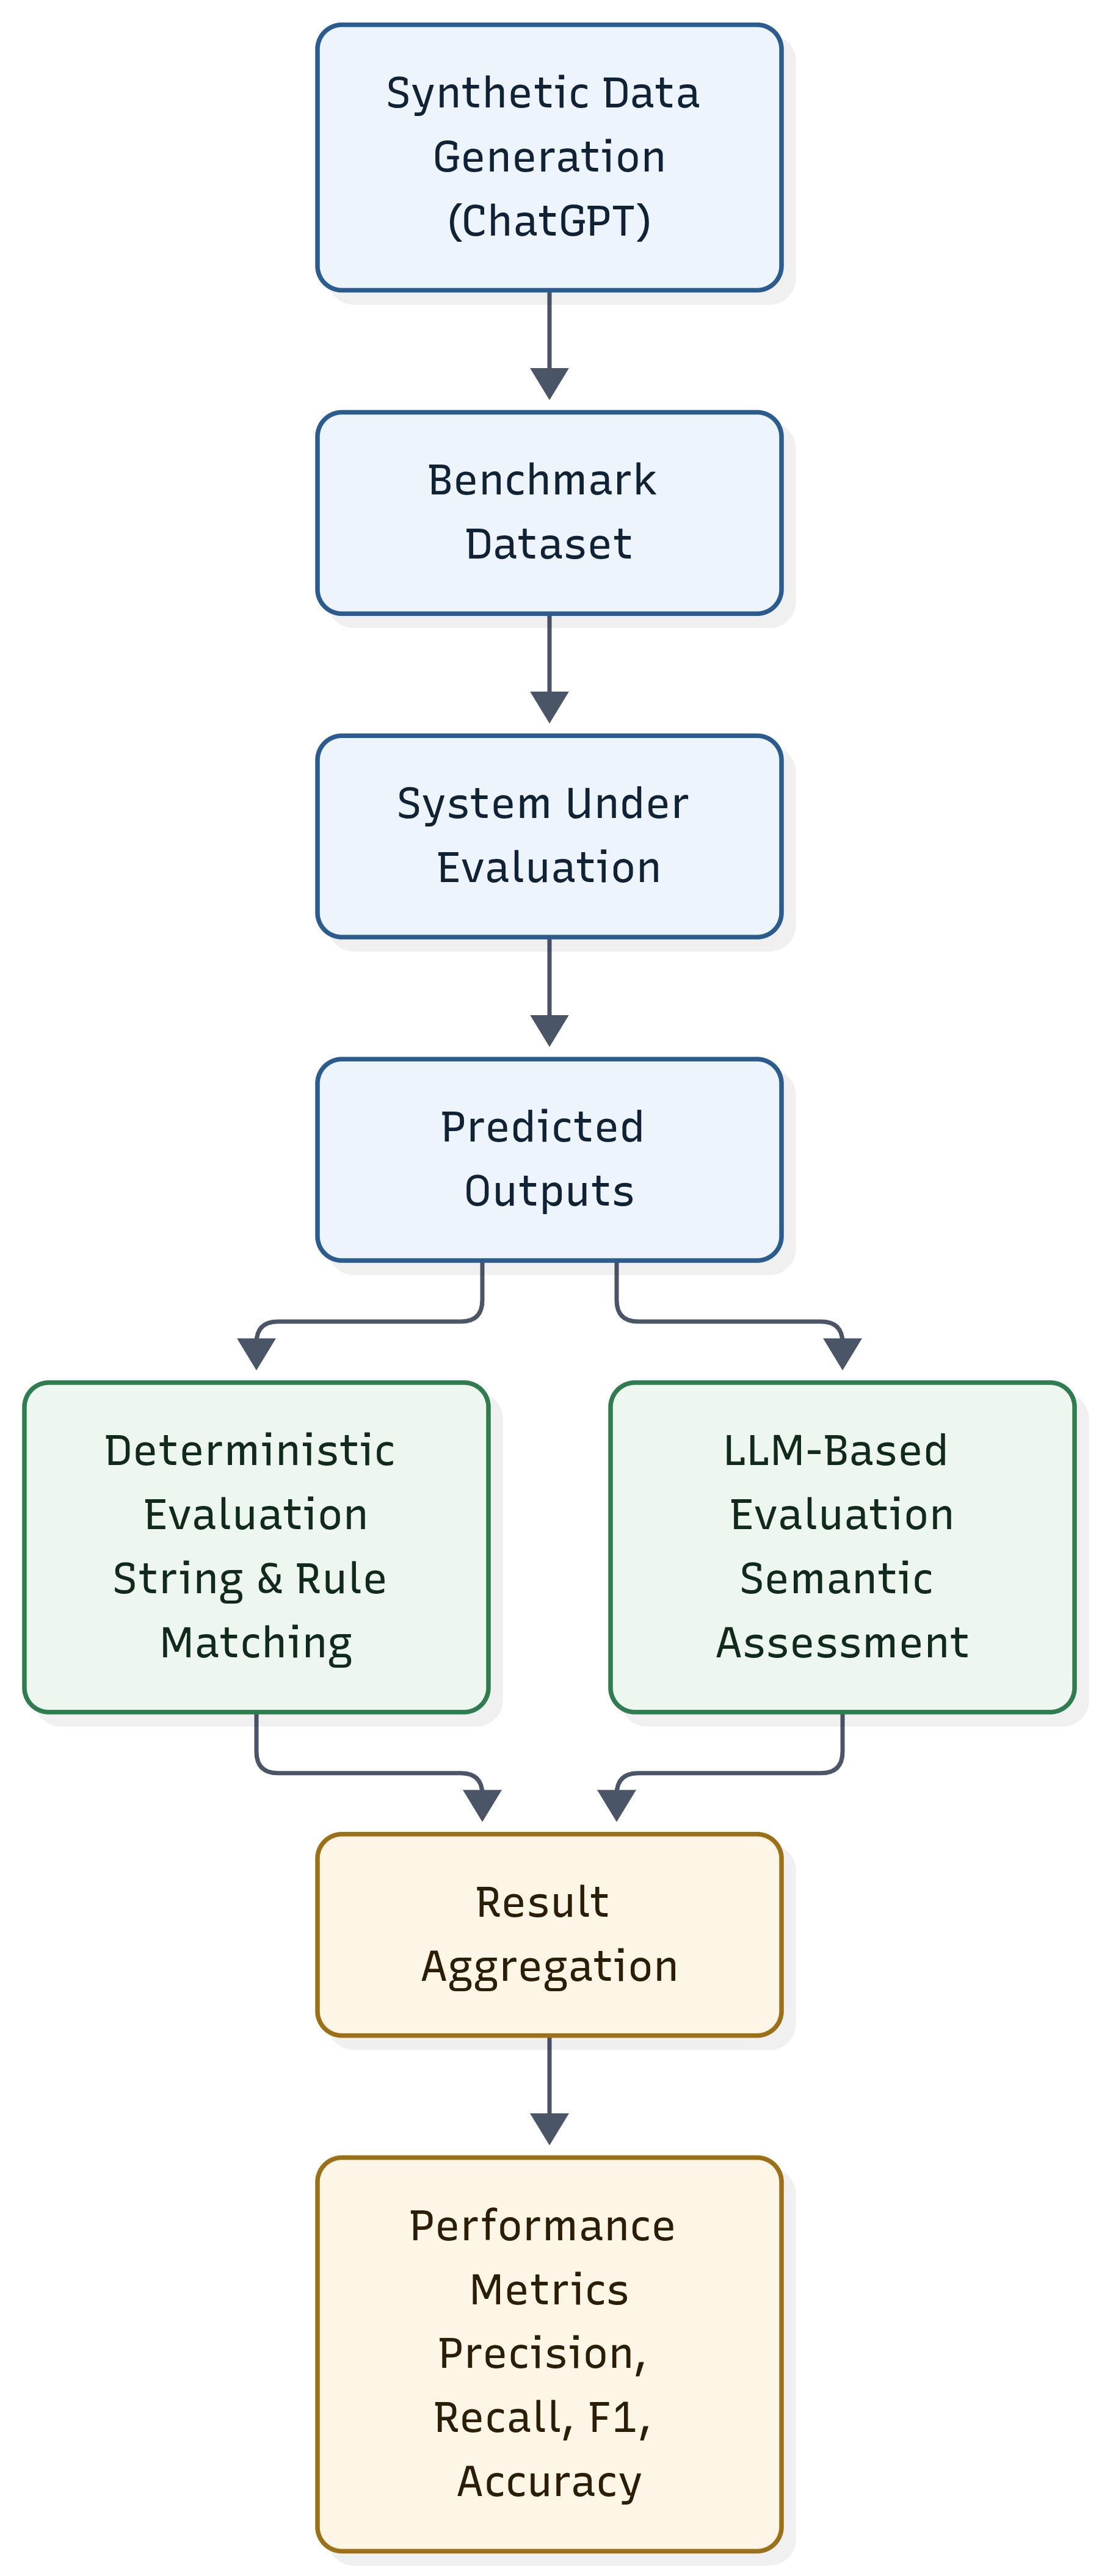
\includegraphics[width=0.41\linewidth]{hybrid_benchmark_flowchart.png}
    \caption{Hybrid Benchmarking framework}
    \label{fig:hybrid_benchmark_flowchart}
\end{figure}
\subsubsection{Episode Detection Benchmark}
The benchmark evaluates the system's ability to create, continue, close, or skip episodes using 50 test cases. It covers both the Turn Analyzer and the episode-handling logic in the orchestrator.

As shown in Table~\ref{tab:episode_detection}, the system performed well across all four actions. Most errors involved distinguishing between ongoing and resolved episodes, suggesting that identifying when an experience has ended remains a challenge.

\begin{table}[!ht]
\centering
\footnotesize
\renewcommand{\arraystretch}{1.4}
\setlength{\tabcolsep}{8pt}
\begin{tabular}{|l|c|c|c|}
\hline
\textbf{Action} & \textbf{Prec.} & \textbf{Recall} & \textbf{F1} \\ \hline
CREATE   & 1.000 & 0.900 & 0.947 \\ \hline
NONE     & 0.909 & 1.000 & 0.952 \\ \hline
CONTINUE & 0.882 & 1.000 & 0.938 \\ \hline
CLOSE    & 1.000 & 0.867 & 0.929 \\ \hline
Accuracy & \multicolumn{3}{c|}{94\%} \\ \hline
Macro F1 & \multicolumn{3}{c|}{0.9415} \\ \hline
\end{tabular}
\renewcommand{\arraystretch}{1}
\setlength{\tabcolsep}{6pt}
\caption{Episode Detection Benchmark Results}
\label{tab:episode_detection}
\end{table}

\subsubsection{Turn Analyzer Benchmark}
The benchmark evaluates the Turn Analyzer's ability to classify user moods and identify meaningful reflections across 50 test cases. As shown in Tables~\ref{tab:mood_results} and~\ref{tab:reflection_results}, mood classification showed stronger performance for some categories, while neutral mood detection remained challenging. Reflection detection achieved perfect recall but lower precision, indicating that some ordinary statements were incorrectly identified as reflections.The evaluation results are presented in Table~\ref{tab:mood_results} and Table~\ref{tab:reflection_results}.

\subsubsection{Long-Term Memory Benchmark}
The Long-Term Memory benchmark evaluates the system's ability to consolidate information from previous memory, episode summaries, mood observations, reflections, and validated patterns into updated memory. It uses 10 test cases covering memory consolidation, pattern-informed updates, memory retention, corrections, and situations with insufficient evidence. The generated memories are assessed using two independent approaches. A rule-based evaluator examines fact precision, fact recall, hallucination, and retention using lexical matching and structural checks. An LLM-based judge evaluates factual support, expected fact coverage, preservation of previous information, correction handling, validated pattern handling, temporary mood handling, reflection usefulness, and resolved pattern handling. Both evaluations are performed against the expected memory and the evidence provided in each test case. The evaluation results are presented in Table~\ref{tab:long_term_memory}.
\begin{table}[!ht]
\centering
\footnotesize
\renewcommand{\arraystretch}{1.4}
\setlength{\tabcolsep}{7pt}
\begin{tabular}{|l|c|}
\hline
\textbf{Metric} & \textbf{Score} \\ \hline
Total Test Cases & 10 \\ \hline
Generation Completed & 10 \\ \hline
Generation Failed & 0 \\ \hline
Rule-based Evaluation Completed & 10 \\ \hline
LLM Judge Evaluation Completed & 10 \\ \hline
Fact Precision (Heuristic) & 0.3375 \\ \hline
Fact Recall (Heuristic) & 0.6750 \\ \hline
Hallucination Rate (Heuristic) & 0.0875 \\ \hline
Retention Accuracy (Heuristic) & 0.9630 \\ \hline
Factual Support (LLM Judge) & 0.9810 \\ \hline
Expected Fact Coverage & 0.9500 \\ \hline
Previous Memory Preservation & 0.9400 \\ \hline
Explicit Correction Handling & 1.0000 \\ \hline
Validated Pattern Handling & 1.0000 \\ \hline
Temporary Mood Handling & 0.8000 \\ \hline
Reflection Usefulness & 0.8000 \\ \hline
Resolved Pattern Handling & 0.8889 \\ \hline
Overall Quality (LLM Judge) & 0.9150 \\ \hline
\end{tabular}
\renewcommand{\arraystretch}{1}
\setlength{\tabcolsep}{6pt}
\caption{Long-Term Memory Benchmark Results}
\label{tab:long_term_memory}
\end{table}

\begin{table}[!ht]
\centering
\footnotesize
\renewcommand{\arraystretch}{1.4}
\setlength{\tabcolsep}{8pt}
\begin{tabular}{|l|c|c|c|}
\hline
\textbf{Mood / Metric} & \textbf{Prec.} & \textbf{Recall} & \textbf{F1} \\ \hline
Angry    & 0.857 & 0.857 & 0.857 \\ \hline
Disgust  & 1.000 & 0.800 & 0.889 \\ \hline
Fear     & 0.889 & 1.000 & 0.941 \\ \hline
Happy    & 1.000 & 1.000 & 1.000 \\ \hline
Neutral  & 1.000 & 0.083 & 0.154 \\ \hline
Sad      & 0.778 & 0.875 & 0.824 \\ \hline
Surprise & 1.000 & 0.800 & 0.889 \\ \hline
\multicolumn{4}{|l|}{\textbf{Total Test Cases: 50}} \\ \hline
\multicolumn{4}{|l|}{\textbf{Completed: 49 \quad Failed: 1}} \\ \hline
\multicolumn{4}{|l|}{\textbf{Mood Accuracy: 0.6939}} \\ \hline
\multicolumn{4}{|l|}{\textbf{Macro F1-score: 0.6942}} \\ \hline
\end{tabular}
\renewcommand{\arraystretch}{1}
\setlength{\tabcolsep}{6pt}
\caption{Turn Analyzer Mood Classification Results}
\label{tab:mood_results}
\end{table}

\begin{table}[!ht]
\centering
\footnotesize
\renewcommand{\arraystretch}{1.4}
\setlength{\tabcolsep}{8pt}
\begin{tabular}{|l|c|}
\hline
\textbf{Metric} & \textbf{Score} \\ \hline
Precision & 0.500 \\ \hline
Recall    & 1.000 \\ \hline
F1-score  & 0.667 \\ \hline
\end{tabular}
\caption{Turn Analyzer Reflection Detection Results}
\label{tab:reflection_results}
\end{table}

\subsubsection{Pattern Memory Benchmark}
The benchmark evaluates the system's ability to identify and maintain recurring patterns across episodes, including pattern updates, reactivation, resolution, and semantic merging. It also examines how well the analyzer supports its identified patterns with evidence from previous episodes and avoids identifying overly broad associations when no specific pattern is expected.
The evaluation results are presented in Table~\ref{tab:pattern_memory}.
\begin{table}[!ht]
\centering
\footnotesize
\renewcommand{\arraystretch}{1.4}
\setlength{\tabcolsep}{7pt}
\begin{tabular}{|l|c|}
\hline
\textbf{Metric} & \textbf{Score} \\ \hline
Total Test Cases & 50 \\ \hline
Cases with Expected Patterns & 40 \\ \hline
Completed and Scored Cases & 37 \\ \hline
Failed Cases & 3 \\ \hline
True Positives (TP) & 32 \\ \hline
False Negatives (FN) & 5 \\ \hline
Recall & 0.8649 \\ \hline
Evidence Quote Validity & 1.0000 \\ \hline
Mean Evidence Episode Coverage & 0.6847 \\ \hline
Lifecycle Accuracy & 0.96875 \\ \hline
Pattern ID Accuracy & 1.0000 \\ \hline
\end{tabular}
\renewcommand{\arraystretch}{1}
\setlength{\tabcolsep}{6pt}
\caption{Pattern Memory Benchmark Results}
\label{tab:pattern_memory}
\end{table}


\subsubsection{Knowledge RAG Benchmark}
The Knowledge RAG benchmark evaluates the system's ability to retrieve relevant information and generate answers grounded in the retrieved content. A dataset of 41 questions was used, each containing a reference answer and supporting evidence phrases. The knowledge base included curated resources such as NICE guidelines on depression, anxiety, and PTSD, WHO mental health publications, and psychological intervention manuals. For retrieval evaluation, the production \textbf{LocalRetriever} was used, combining ChromaDB vector search and BM25 keyword search through Reciprocal Rank Fusion (RRF). Ground-truth chunks were identified using BGE embedding similarity against the evidence phrases and graded by GPT-OSS 120B based on their relevance to the expected answers.

For answer evaluation, the system generated responses using the top five retrieved chunks for each question. The generated answers were compared with the reference answers using BGE cosine similarity and an LLM-based judge, which assessed their correctness and supporting evidence. The results of both evaluations are presented in Table~\ref{tab:knowledge_rag}.
\begin{table}
\centering
\footnotesize
\renewcommand{\arraystretch}{1.4}
\setlength{\tabcolsep}{7pt}
\begin{tabular}{|l|c|}
\hline
\textbf{Metric} & \textbf{Score} \\ \hline
Total Questions & 41 \\ \hline
Retrieval-Evaluable Questions & 39 \\ \hline
Not Evaluated for Retrieval & 2 \\ \hline
Precision@3 & 0.4444 \\ \hline
Recall@3 & 0.3097 \\ \hline
nDCG@3 & 0.4907 \\ \hline
Precision@5 & 0.3590 \\ \hline
Recall@5 & 0.4176 \\ \hline
nDCG@5 & 0.4983 \\ \hline
Precision@10 & 0.2462 \\ \hline
Recall@10 & 0.5792 \\ \hline
nDCG@10 & 0.5323 \\ \hline
MRR@10 & 0.7879 \\ \hline
Mean BGE Cosine Similarity & 0.7572 \\ \hline
LLM Exact-Correct Rate & 0.8537 \\ \hline
LLM Weighted Answer Score & 0.9024 \\ \hline
\end{tabular}
\renewcommand{\arraystretch}{1}
\setlength{\tabcolsep}{6pt}
\caption{Knowledge RAG Benchmark Results}
\label{tab:knowledge_rag}
\end{table}
\subsubsection{Conversation-Level Evaluation}
Conversation-level evaluation assesses the chatbot's overall response quality across multi-turn interactions. Complete conversations are evaluated using an LLM-based \textbf{Claude Sonnet 5.5} \cite{claude_sonnet} as the judge, based on four key metrics: \textbf{emotional understanding}, \textbf{empathy and support}, \textbf{contextual relevance}, and \textbf{helpfulness and guidance}. Each metric is rated on a five-point scale, with scores reflecting the chatbot's ability to recognize user emotions, provide empathetic responses, maintain conversational context, and offer relevant and practical guidance. The evaluation also includes a brief qualitative summary of each conversation to highlight the chatbot's strengths and limitations.
The results of evaluations are presented in Table~\ref{tab:conversation_evaluation}.
\begin{table*}[ht]
\centering
\renewcommand{\arraystretch}{1.4}
\small
\begin{tabularx}{\textwidth}{
|>{\raggedright\arraybackslash}X|
>{\raggedright\arraybackslash}p{0.32\textwidth}|
}
\hline
\textbf{Conversation Summary} & \textbf{Evaluation Metrics} \\
\hline

The user reports being unable to relax and feeling mentally exhausted due to minor unfinished tasks, such as replying to a friend, organizing files, and returning a borrowed item. The chatbot suggests writing tasks down and completing them within a short scheduled slot. The approach is practical and relevant, but emotional validation and exploration of the underlying concern are limited.
&
\textbf{Emotional Understanding:} 3/5 \par
\textbf{Empathy and Support:} 3/5 \par
\textbf{Contextual Relevance:} 4/5 \par
\textbf{Helpfulness and Guidance:} 4/5
\\
\hline

The user reports procrastinating on a programming assignment due Friday, as the prospect of spending hours coding feels overwhelming. The chatbot suggests a 20-minute starting session, which the user accepts and finds encouraging. However, subsequent replies become repetitive and do not explore the broader pattern of procrastination.
&
\textbf{Emotional Understanding:} 4/5 \par
\textbf{Empathy and Support:} 3/5 \par
\textbf{Contextual Relevance:} 4/5 \par
\textbf{Helpfulness and Guidance:} 4/5
\\
\hline

The user describes frequent replaying of conversations and overthinking, leading to distraction, phone checking, and delayed assignments. The chatbot suggests a five-minute daily reflection routine, which the user accepts. Although relevant, it does not adequately address the underlying fear of upsetting others or the phone-checking behavior.
&
\textbf{Emotional Understanding:} 4/5 \par
\textbf{Empathy and Support:} 3/5 \par
\textbf{Contextual Relevance:} 4/5 \par
\textbf{Helpfulness and Guidance:} 3/5
\\
\hline

The user reports repeatedly checking email while awaiting an important reply, disrupting study and work, alongside difficulty starting lengthy assignments. The chatbot recommends fixed email-checking windows and short breaks. However, it does not sufficiently explore the underlying worry or provide strategies for managing lengthy tasks.
&
\textbf{Emotional Understanding:} 2/5 \par
\textbf{Empathy and Support:} 3/5 \par
\textbf{Contextual Relevance:} 3/5 \par
\textbf{Helpfulness and Guidance:} 3/5
\\
\hline

The user, an intern balancing college and assignments, fears receiving a midnight email from their boss and repeatedly checks their inbox, followed by procrastination and watching reels. The chatbot suggests fixed email windows, an auto-reply, and timed study sessions. While practical, it overlooks workplace constraints and does not adequately explore the underlying anxiety.
&
\textbf{Emotional Understanding:} 3/5 \par
\textbf{Empathy and Support:} 3/5 \par
\textbf{Contextual Relevance:} 3/5 \par
\textbf{Helpfulness and Guidance:} 3/5
\\
\hline

\end{tabularx}
\caption{Qualitative Evaluation of Mental Health Chatbot Conversations}
\label{tab:conversation_evaluation}
\end{table*}
\subsection{Modularity and Extensibility}
The proposed system follows a modular architecture, allowing individual components to be modified and improved independently without requiring major changes to the overall implementation. Each LLM-based component uses dedicated prompts that can be adjusted to change its behaviour, refine its decision-making, and improve its outputs. The system also supports flexibility in selecting the underlying LLM, allowing different models and providers to be integrated with minimal changes to the implementation. This makes it easier to experiment with newer models, refine component behaviour, and extend the system with additional capabilities as requirements evolve.
\subsection{Limitations}
The proposed system has several limitations:
\begin{itemize}
    \item \textbf{Episode Management:} Episode creation and closure depend on identifying appropriate conversational cues. Direct expressions of resolution are easier to interpret, whereas indirect expressions may be overlooked. The current approach can also be strict, requiring sufficiently clear indications before closing an episode.

    \item \textbf{Token Consumption:} Multiple LLM calls for mood analysis, episode management, pattern detection, memory consolidation, knowledge retrieval, and response generation make the system relatively token-intensive, increasing API costs and response latency.

    \item \textbf{Benchmark Limitations:} Synthetic test cases and predefined evaluation criteria may not fully represent real-world conversations, where users express themselves ambiguously, change topics unexpectedly, or provide incomplete information.

    \item \textbf{LLM Reliability:} The system may generate inaccurate or fabricated information, misinterpret user messages, or confidently defend incorrect responses. Retrieval grounding and validation mechanisms help reduce these issues but cannot eliminate them entirely.


    \item \textbf{Knowledge Retrieval and Memory Reliability:} The quality of RAG responses depends on the coverage, accuracy, and relevance of the indexed documents. Hybrid retrieval may fail to identify relevant information due to differences in terminology, ranking limitations, or document chunking. Even when relevant content is retrieved, the LLM may misinterpret it or generate unsupported claims. Similarly, long-term memory consolidation may omit important details, retain outdated information, or inaccurately summarize user experiences, affecting the context used in future interactions.

    
    \item \textbf{Pattern Detection:} Identifying recurring patterns requires sufficient evidence across multiple episodes. Limited or inconsistent conversation history may result in missed patterns or incorrect associations.

    \item \textbf{External Dependencies:} The system depends on external API availability and is subject to rate limits, service interruptions, and model-specific behaviour. Changes in model versions may also affect output consistency.

    \item \textbf{Clinical Limitations:} The chatbot is intended for conversational mental health support and is not a substitute for professional assessment, diagnosis, or treatment. Its responses should not be considered clinically validated advice.

    \item \textbf{Limited Real-World Evaluation:} The system has not yet been extensively evaluated through long-term real-world user studies, limiting the assessment of its reliability and usefulness in practical settings.
\end{itemize}
\section{Future Scope}

The proposed system can be further extended in the following directions:

\begin{itemize}
    \item \textbf{Newer LLM Integration:} Integrate newer LLMs as they become available to benefit from improved reasoning and contextual understanding with minimal architectural changes.

    \item \textbf{Fine-Tuned Mental Health Models:} Explore models fine-tuned on curated mental health datasets to improve domain-specific understanding and response quality.

    \item \textbf{Modular Enhancements:} Add, remove, or refine individual components and optimize their prompts to improve behaviour and decision-making.

    \item \textbf{Advanced RAG:} Explore Graph RAG to capture relationships between mental health concepts, along with improved reranking, query expansion, and retrieval strategies.

    \item \textbf{Enhanced Personalization:} Improve memory mechanisms to better capture evolving experiences, behavioural patterns, preferences, and coping strategies.

    \item \textbf{Multimodal Interaction:} Introduce voice-based interactions and other input modalities to incorporate additional contextual information.

    \item \textbf{Multilingual Support:} Extend the system to support multiple languages and enable interactions in users' preferred languages.

    \item \textbf{Safety and Evaluation:} Strengthen crisis detection and response safeguards, and conduct further evaluation with real-world users over a longer period.
\end{itemize}

\section{Conclusion}

This paper presented a personalized mental health chatbot designed to provide context-aware support across multiple conversations. It combines LLM-based processing with episodic memory, mood and reflection tracking, pattern identification, and long-term memory consolidation to understand users' experiences over time. A Knowledge RAG component further supports responses by retrieving relevant information from curated mental health resources.

The system's modular architecture allows components to be refined through dedicated prompts and different LLMs to be integrated with minimal changes. Component-level benchmarks evaluated episode detection, mood and reflection analysis, pattern identification, long-term memory consolidation, and knowledge retrieval. The results highlight the potential of combining conversational memory and knowledge retrieval for personalized interactions, while identifying areas for improvement. The system provides a foundation for adaptive mental health chatbots, with scope for improvements in models, retrieval, memory, safety, and real-world evaluation.

The complete project implementation and benchmark test datasets are publicly available on GitHub \cite{mentalhealthchatbot}, providing resources for further inspection and evaluation.

\section*{Acknowledgment}
The authors acknowledge the use of ChatGPT by OpenAI \cite{chatgpt} to assist with language refinement, grammar correction, and improving the clarity of the manuscript. All technical content, implementation, analysis, and conclusions were reviewed and verified by the authors.

\begin{thebibliography}{00}
\bibitem{b1} R. S. Ponmagal, H. Deep, and D. Yadav, 
``Mental Health Support Using Gen-AI Shot Prompting Technique and Vector Embeddings,''
in \textit{Proc. 2025 International Conference on Data Science and Business Systems (ICDSBS)}, 2025, pp. 1--5, 
doi: 10.1109/ICDSBS63635.2025.11031881.
\bibitem{b2} S. Jaybhaye, S. Deogade, S. Sanap, T. Mali, and U. Shendge, ``BlissBot: Mental Health Chatbot,'' in Proc. 2024 IEEE Region 10 Symposium (TENSYMP), 2024, doi: 10.1109/TENSYMP61132.2024.10752315.

\bibitem{b3} B. P. Prathaban, R. Subash, and A. Ashwini, ``AI Based Mental Health Assisted Chatbot System,'' in Proc. 2024 International Conference on Power, Energy, Control and Transmission Systems (ICPECTS), 2024, doi: 10.1109/ICPECTS62210.2024.10780017.

\bibitem{b4} A. Verma, B. Sruthi, and S. Rajashree, ``Calm Companion -- An Enhanced Chatbot for Mental Health Support,'' in Proc. 2025 5th International Conference on Expert Clouds and Applications (ICOECA), 2025, doi: 10.1109/ICOECA66273.2025.00046.

\bibitem{b5} J. Sophia, K. Manoharan, and K. Arul, ``Evaluation of BERT and BART in Mental Health Dialogue by Using a Counselling Chatbot,'' in Proc. 2025 International Conference on Engineering Innovations and Technologies (ICoEIT), 2025, doi: 10.1109/ICOEIT63558.2025.11211681.

\bibitem{b6} G. B. Nair, A. Krishnan, and V. G., ``Adaptive Chatbot for Mental Health Screening and Personalized Self-Help Interventions,'' in Proc. 2026 International Conference on Advancements in Smart, Secure and Intelligent Computing (ASSIC), 2026, doi: 10.1109/ASSIC70037.2026.11717149.

\bibitem{b7}
S. Bagal, S. Pise, R. Netke, and T. Narokar,
``AIMind: An AI-Powered Framework for Personalized Mental Health Support,''
in \textit{Proc. 18th International Conference on Electronics, Computers and Artificial Intelligence (ECAI)}, 2026, pp. 1--9,
doi: 10.1109/ECAI69016.2026.11613794.

\bibitem{b8}
R. Mavila, S. Jaiswal, R. Naswa, W. Yuwen, B. Erdly, and D. Si,
``iCare -- An AI-Powered Virtual Assistant for Mental Health,''
in \textit{Proc. 2024 IEEE 12th International Conference on Healthcare Informatics (ICHI)}, 2024, pp. 466--471,
doi: 10.1109/ICHI61247.2024.00066.

\bibitem{b9}
C. Jewell, K. McAlister, T. Deliberto, T. Wallis, G. Winns, and J. Huberty,
``From Personalization to Therapeutic Continuity: Framework for Memory in AI-Powered Mental Health Systems,''
\textit{JMIR AI}, vol. 5, 2026, Art. no. e99950,
doi: 10.2196/99950.

\bibitem{b10}
G. Hao, Y. Zhang, G. Ma, Y. Chen, F. Alexandre, and S. Yu,
``Large Language Models Need Episodic Memory,''
in \textit{Proc. International Joint Conference on Neural Networks (IJCNN)}, Rome, Italy, Jun. 2025.

\bibitem{b11}
W. K. C. Leung, S. C. Lam, B. C. L. Chan, J. N. L. Chow, Y. Y. Y. Wong, F. Ng, C. C. K. Yip, and A. C. K. Chan,
``Chatbot interventions for improving mental health among people in Asia: A systematic review and meta-analysis of randomised controlled trials,''
\textit{BMJ Health Care Informatics}, vol. 33, Art. no. e101479, 2026,
doi: 10.1136/bmjhci-2025-101479.

\bibitem{mentalhealthchatbot}
P. G. N. Pranav, ``Mental Health Chatbot,'' GitHub repository. [Online]. Available: \url{https://github.com/pranavgn12/mental-health-chatbot}. Accessed: Nov. 26, 2026.

\bibitem{claude_sonnet}
Anthropic, ``Claude Sonnet 5.5,'' [Online]. Available: 
\url{https://www.anthropic.com/claude-sonnet-5-5}. Accessed: Nov. 26, 2026.

\bibitem{chatgpt}
OpenAI, ``ChatGPT,'' [Online]. Available:
\url{https://chatgpt.com/}. Accessed: Nov. 26, 2026.
\bibitem{gpt_oss}
OpenAI, ``Introducing gpt-oss,'' Aug. 5, 2025. [Online]. Available:
\url{https://openai.com/index/introducing-gpt-oss/}. Accessed: Nov. 26, 2026.

\bibitem{groq}
Groq, ``Groq,'' [Online]. Available:
\url{https://groq.com/}. Accessed: Nov. 26, 2026.
\end{thebibliography}
\end{document}
